% !TEX root = ../notes_template.tex

\chapter{코시 적분 정리와 응용}

복소미분은 어느정도 익숙해졌으니 이제 적분으로 관심을 돌려보자.
이 장에서는 복소해석학에서 매우 중요한 다음 정리를 배울 예정이다.
\begin{center}
\fbox{
코시 적분 정리
}
\end{center}
``경로적분''을 정의하는 것으로 시작하여 나중에 코시 적분 정리를 증명할 예정이다.
왜 경로적분과 코시 적분 정리가 왜 그렇게 중요한지 의문을 가질 수 있다.
복소평면에서 적분의 중요성은 복소해석함수의 더 큰 이해로 이어지기 때문이다.
예를 들면, 복소해석함수는 무한번 미분가능하다는 본질적인 성질이 있다.
이 장에서 다음 주제들을 중심으로 공부해보기로 하자.
\begin{enumerate}
\item[(1)] 경로적분의 정의와 성질
\item[(2)] 경로적분의 기본정리
\item[(3)] 코시 적분 정리
\item[(4)] 코시 적분 정리의 응용
\begin{enumerate}
\item 부정적분의 존재성
\item 복소해석함수의 무한번 미분가능성
\item 리우비우 정리와 대수학의 기본정리
\item 모레라 정리
\end{enumerate}
\end{enumerate}

\section{경로적분의 정의}

일반적인 미적분에서 연속함수 $f: [a,b] \to \mathbb R$가 주어질 때
\begin{equation}\label{eq-3-1}
\int_a^b f(x)dx
\end{equation}
의 의미는 명확하다. 이제 이를  일반화하여 복소수까지 확장하고
주어진 복소수 $z$, $w$에 대하여
\[
\int_z^w f(\zeta)d\zeta
\]
에 의미를 부여하길 원한다고 하자.
$z$에서 $w$까지를 어떻게 해석해야 할까?

$\mathbb R$에서 $a<b$이면, 실수 $a$부터  실수 $b$까지
가는 경로는 한가지 뿐이다.  
따라서 실수의 경우는 단지
\begin{itemize}
\item[(1)] $a<b$이고,
\item[(2)] 연속함수 $f:[a,b] \to \mathbb R$
\end{itemize}
의 경우만 생각하면 충분하다.

하지만, $z$와 $w$가 복소평면 위의 점이면
그림 \ref{fig-3-1}과 같이 많은 경로에 대하여 적분을 생각할 수 있다.

\begin{figure}[!h]
\begin{center}
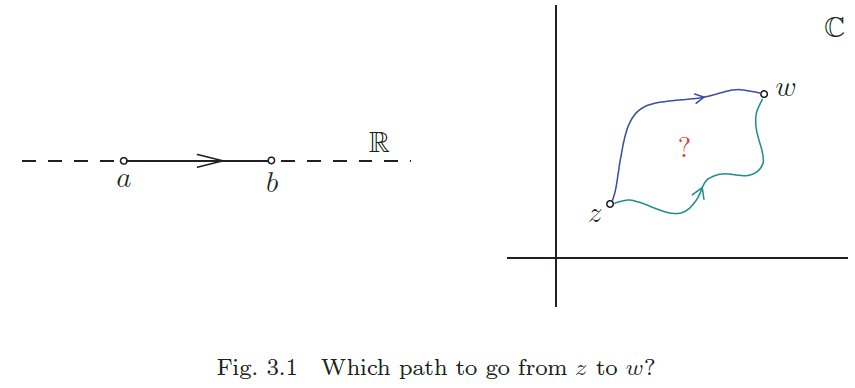
\includegraphics[width=0.8\textwidth]{./SaltChapter/fig-3-1}
\end{center}
\caption{$z$에서 $w$까지 어떤 경로로 가야할까?}
\label{fig-3-1}
\end{figure}

그러므로 복소수의 경우는 끝점 $z$와 $w$ 외에
$z$에서 $w$까지의 경로 $\gamma$도 지정하고,
실수의 경우를 나타낸 식 \eqref{eq-3-1}를
다음과 같이 복소수에 대한 표현으로 바꾸도록 한다.
\[
\int_\gamma f(z)dz.
\]

이 표현을 ``경로''적분이라 부르며
계산을 위해 다음을 결정할 필요가 있다.
\begin{itemize}
\item[(1)] 정의역  $D(\subset \mathbb C)$와 $z, w\in D$
\item[(2)] 연속함수 $f:D\to \mathbb C$
\item[(3)] $z$와 $w$를 잇는 {\bf 매끄러운} 경로 $\gamma: [a,b] \to D$
\end{itemize}

$z$와 $w$를 단순히 연결하는 경로가 아니라  {\bf 매끄러운} 경로가
필요하다는 사실에 주목하자.
여기서 ``매끄럽다''는 의미는 무엇일까?
경로 $\gamma : [a,b] \to D$는 연속함수임을 상기하자.
$\gamma$는 실수부와 허수부 $x,y: [a,b] \to \mathbb R$로 나누어  쓸 수 있다.
\[
\gamma(t) = x(t) + iy(t), \quad t\in [a,b].
\]
$x, y$가 연속미분가능하면
경로 $\gamma$가 {\bf 매끄럽다}고 한다.
예를 살펴보자.

\begin{salt_example} \label{example-3-1}
$\gamma : [0,1] \to \mathbb C$를 
$\gamma(t) = t(1+i)$ ($t\in[0,1]$)로 정의하자.
그러면 $\gamma$의 실수부와 허수부  $x,y: [a,b] \to \mathbb R$는
$x(t)=t$, $y(t)=t$, $t\in [0,1]$이 된다.
$x, y$가 $[0,1]$에서 연속미분가능이므로 $\gamma$는 매끄러운 곡선이다.
그림 \ref{fig-3-2}를 참고하라.
\begin{figure}[!h]
\begin{center}
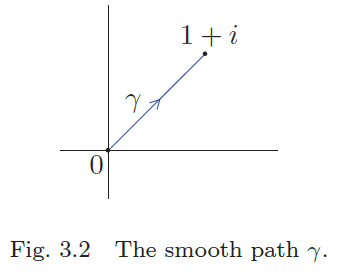
\includegraphics[width=0.4\textwidth]{./SaltChapter/fig-3-2}
\end{center}
\caption{매끄러운 곡선 $\gamma$}
\label{fig-3-2}
\end{figure}
비슷한 방법으로 다음과 같이 주어진 두 경로  $\gamma_1, \gamma_2: [0,2\pi] \to \mathbb R$를
생각하자.
\[
\gamma_1(t) = \exp(it), \quad \gamma_2(t) = \exp(2it), \quad t\in [0,2\pi].
\]
그러면 이 경로들의 실수부와 허수부는
$\cos t$, $\sin t$, $\cos(2t)$, $\sin(2t)$이고
모두 연속미분가능하다.
따라서 $\gamma_1, \gamma_2$는 모두 매끄러운 경로이다.
그림 \ref{fig-3-3}을 보자.
\begin{figure}[!h]
\begin{center}
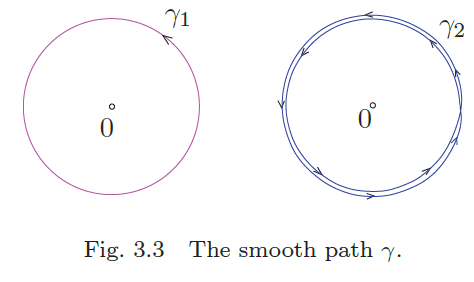
\includegraphics[width=0.6\textwidth]{./SaltChapter/fig-3-3}
\end{center}
\caption{매끄러운 곡선 $\gamma_1$과 $\gamma_2$}
\label{fig-3-3}
\end{figure}
두 곡선의 이미지 ($\gamma_1$과 $\gamma_2$의 치역)은 동일하다.
즉, 중심이 원점인 단위원이다.
\[
\{\gamma_1(t) \,:\, t\in[0,2\pi]\}  
= \{\gamma_2(t) \,:\, t\in[0,2\pi]\}  
= \{z\in\mathbb C \,:\, |z|=1 \}. 
\] 
그렇지만 $\gamma_1$과 $\gamma_2$는 다른 경로이다.
왜냐하면 함수로서 같지 않기 때문이다. 예를 들면
$\gamma_1(\pi) = -1 \ne 1 = \gamma_2(\pi)$.
\hfill $\diamondsuit$
\end{salt_example}

\begin{salt_remark} \label{remark-3-1}
경로 $\gamma: [a,b]\to \mathbb C$의 치역
\[
\{\gamma(t) \,:\, t\in[a,b] \}
\]
을 경로(또는 곡선) 자체라고 하는 것이 매우 일반적이며 편리하다. 
이 방식에서는 경로는 
복소평명에서의 원, 선분 구체적인 기하학적 개체가 되어 (함수라고 생각하는 것과 반대로),
쉽게 그려볼 수 있다.
이 방식에서는 {\bf 다른} 경로를 동일한 이미지로 볼 수 있어
모호함이 생긴다는 어려움이 있다.
\end{salt_remark}

경로적분의 정확한 정의는 다음과 같다.

\begin{salt_definition} \label{def-3-1}
다음이 주어질 때,
\begin{itemize}
\item[(1)] 정의역 $D$,
\item[(2)] 연속함수  $f:D\to\mathbb C$ (실수부와 허수부는 
$u,v: D\to\mathbb R$),
\item[(3)] 매끄러운 경로 $\gamma : [a,b]\to D$
(실수부와 허수부는 $x,y: [a,b] \to \mathbb R$),
\end{itemize}
경로적분을 다음과 같이 정의한다.
\begin{align} \label{eq-3-2}
\int_\gamma f(z)dz
&:= \int_a^b f(\gamma(t))\gamma'(t)dt \\
&:= \int_a^b \left( u(\gamma(t)) + iv(\gamma(t)) \right) \cdot
(x'(t) + iy'(t))dt \nonumber \\
&:= \int_a^b \left( u(\gamma(t)\cdot x'(t) - v(\gamma(t))\cdot y'(t) \right) \nonumber \\
&\quad +i \int_a^b \left(v(\gamma(t)\cdot x'(t) + u(\gamma(t))\cdot y'(t) \right) dt \nonumber.
\end{align}
여기서 마지막 두 적분은 우리에게 익숙한 실변수 연속함수의 리만적분이다.
\end{salt_definition}

다음과 같이 경로적분을 기하학적으로 해석할 수 있다.
\[
\gamma'(t) dt = x'(t)dt + iy'(t)dt
\]
이 항을 경로를 따라 국소적으로 변하는 증분으로 보자.
이 증분에 값 $f(\gamma(t))$ (국소적으로는 거의 상수이다)을 곱하고,
경로를 따라 더해나가면 결론적으로 적분값
\[
\int_a^b f(\gamma(t))\gamma'(t)dt
\]
에 도달하게 된다. 그림 \ref{fig-3-4}를 참고하라.

\begin{figure}[!h]
\begin{center}
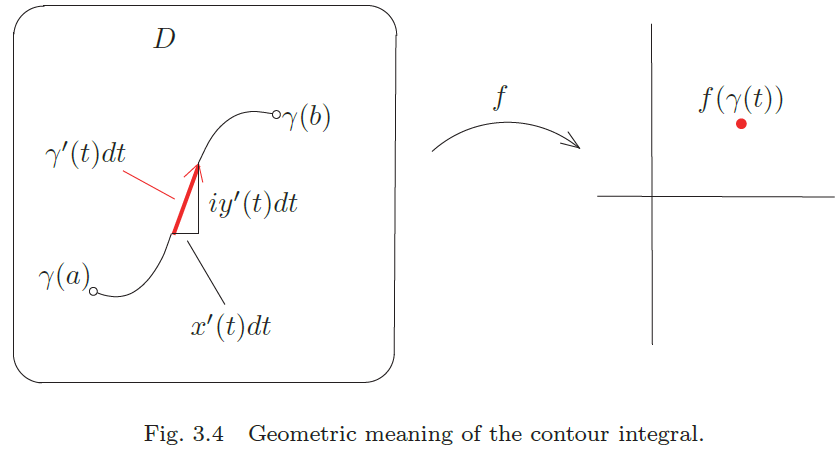
\includegraphics[width=0.8\textwidth]{./SaltChapter/fig-3-4}
\end{center}
\caption{경로적분의 기하학적 의미}
\label{fig-3-4}
\end{figure}

\begin{salt_example} \label{example-3-2}
다음과 같이 주어진 조건에 대하여
\begin{itemize}
\item[(1)] $D=\mathbb C$,
\item[(2)] $\gamma$는 $\gamma(t)= t(1+i)$ ($t\in[0,1]$)로 정의된 매끄러운 경로,
\item[(3)] $f = (z\to \bar z)$,
\end{itemize}
\begin{align*}
\int_\gamma f(z)dz &= \int_0^1 \overline{t(1+i)}\cdot (1+i)dt \\
&= \int_0^1 t(1-i)\cdot(1+i)dt
= \int_0^1 t(1^2-i^2)dt = \int_0^1 t(1+1)dt \\
&= 2\int_0^1 t\,dt = 2\cdot \frac{t^2}2 \Big|_0^1 = 2\cdot \dfrac12 = 1.
\end{align*}
\end{salt_example}

\begin{salt_exercise} \label{ex-3-1}
세 경로 $\gamma_1, \gamma_2, \gamma_3: [0,2\pi] \to \mathbb C$가 
$t\in[0,2\pi]$에 대하여 다음과 같이 정의된다고 하자.
\begin{align*}
\gamma_1(t) &= \exp(it), \\
\gamma_2(t) &= \exp(2it), \\
\gamma_3(t) &= \exp(-it).
\end{align*}
경로의 이미지는 모두 같지만, 다음 세 경로적분은 모두 다른 값을 가짐을 보여라.
\[
\int_{\gamma_1} \dfrac1zdz, \quad
\int_{\gamma_2} \dfrac1zdz, \quad
\int_{\gamma_3} \dfrac1zdz.
\]
\end{salt_exercise}

\begin{salt_exercise} \label{ex-3-2}
$f$가 영역 $D$에서 복소해석함수이고, $\gamma:[0,1]\to D$가 매끄러운 경로라 하자.
모든 $t\in[0,1]$에 대하여 다음을 증명하라.
\[
\dfrac{d}{dt} f(\gamma(t)) = f'(\gamma(t))\cdot \gamma'(t). 
\]
\end{salt_exercise}

우리는 종종 일반적인 구간 $[a,b]$를 사용하지 않고
매끄러운 경로가 $[0,1]$에서 매개변수로 정의된 것으로 가정하기도 한다.
왜 이런 가정을 해도 되는지 이유를 설명해보자.

$\gamma:[a,b] \to \mathbb C$와  $\tilde\gamma:[a,b] \to \mathbb C$가
매끄러운 경로라고 하자.
연속미분가능한 함수 $\varphi:[c,d] \to [a,b]$가
$a=\varphi(c)$, $b=\varphi(d)$이고 모든 $t\in[c,d]$에 대하여
$\tilde\gamma(t) = \gamma(\varphi(t))$를 만족한다고 하자.
이러한 두 경로를 ``동치''라고 한다.
$\gamma(a) = \tilde\gamma(c)$부터 $\gamma(b) = \tilde\gamma(d)$까지
동일한 길을 따라 간다고 상상해보자. 단, 속도는 다를 수 있다.
그림 \ref{fig-3-5}를 보자. 
\begin{figure}[!h]
\begin{center}
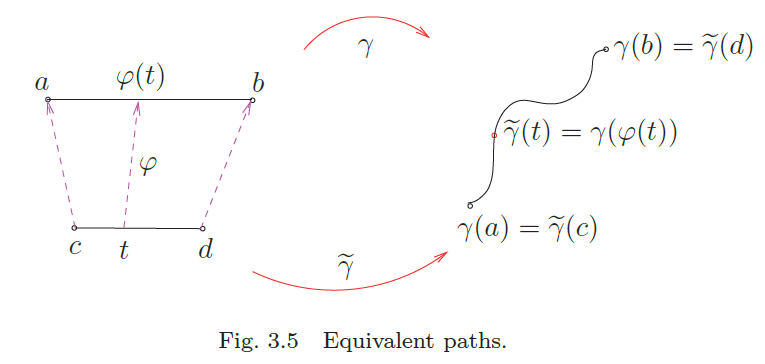
\includegraphics[width=0.7\textwidth]{./SaltChapter/fig-3-5}
\end{center}
\caption{동치 경로}
\label{fig-3-5}
\end{figure}
이제 다음 결과를 보일 수 있다.

{\bf 동치 경로에 대한 적분결과는 동일하다:}
연쇄법칙에 의해 다음이 성립한다.
\begin{align*}
\int_{\tilde\gamma}f(z)dz
&= \int_c^d f(\tilde\gamma(t))\tilde\gamma'(t)dt
= \int_c^d f(\gamma(\varphi(t)))\gamma'(\varphi(t)) \varphi'(t)dt \\
&\stackrel{(\tau=\varphi(t))}=
\int_a^b f(\gamma(\tau))\gamma'(\tau)d\tau
= \int_{\gamma}f(z)dz.
\end{align*}
특히, 주어진 $\gamma:[a,b]\to\mathbb C$에 대하여
$\varphi: [0,1]\to [a,b]$를 다음과 같이 정의하자.
\[
\varphi(t) = (1-t)a + tb, \quad t\in [a,b].
\]
그러면 $\varphi$는 연속미분가능하고,
$\varphi(0)=a$, $\varphi(1)=b$이다.
따라서 $c:=0$, $d:=1$로 두고 위의 결과를 적용하면,
$\tilde\gamma : [0,1]\to\mathbb C$를
$\tilde\gamma = \gamma\circ\varphi$라 정의하여
다음을 얻는다.
\[
\int_{\tilde\gamma} f(z)dz = \int_\gamma f(z)dz.
\]
결론적으로, 경로적분과 관련하여
매끄러운 곡선은 $[0,1]$에서 매개화된 것으로 간주해도 일반성을 잃지 않는다.

{\bf 조각적으로 매끄러운 경로에 대한 경로적분:}
경로의 정의를 ``꺽인 점''을 갖는 경로까지 확장해보자.
점 $c_1, \ldots, c_n$가
\[
a<c_1 < \cdots <c_n <b
\]
를 만족하고 $\gamma$가 구간 $[a,c_1], [c_1,c_2], \ldots, [c_{n_1}, c_n], [c_n,b]$ 각각에서
연속미분가능할 때,
경로 $\gamma:[a,b]\to\mathbb C$가 {\bf 조각적으로 매끄러운 경로 또는 곡선}이라 한다.
이러한 경로에서의 적분은 다음과 같이 정의한다.
\begin{align*}
\int_\gamma f(z)dz
&:= \int_a^{c_1} f(\gamma(t))\gamma'(t)dt + \int_{c_1}^{c_2} f(\gamma(t))\gamma'(t)dt
+ \cdots \\
&\quad \quad + \int_{c_{n-1}}^{c_n} f(\gamma(t))\gamma'(t)dt 
+ \int_{c_n}^b f(\gamma(t))\gamma'(t)dt.
\end{align*}

\begin{salt_example} \label{example-3-3}
$0$부터 $1+i$까지의 경로 $\tilde\gamma$가 다음과 같이 정의된다고 하자.
\[
\tilde\gamma(t) = \begin{cases}
t, & t\in[0,1], \\
1+(t-1)i, t\in (1,2].
\end{cases}
\]
그림 \ref{fig-3-6}을 보자.
\begin{figure}[!h]
\begin{center}
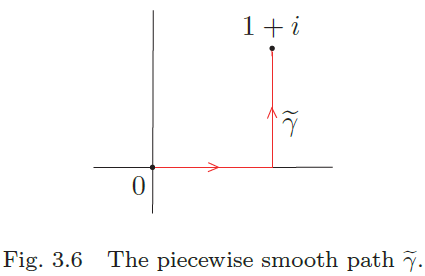
\includegraphics[width=0.4\textwidth]{./SaltChapter/fig-3-6}
\end{center}
\caption{조각적으로 매끄러운 경로 $\tilde\gamma$}
\label{fig-3-6}
\end{figure}
그러면
\begin{align*}
\int_{\tilde\gamma} \bar z dz 
&= \int_0^1 \bar t \,1\,dt
+ \int_1^2 \overline{(1+(t-1)i)}\,i\, dt
= \int_0^t t\,dt + \int_1^2 (1-(t-1)i)i\,dt \\
&= \int_0^1 t\,dt + \int_1^2 (i+(t-1))dt \\
&= \dfrac12 + i + \dfrac{4-1}2 - 1 = 1+ i.
\end{align*}
\end{salt_example}

예제 \ref{example-3-2}와 \ref{example-3-3}에서 얻은 계산결과를 돌아보자.
피적분함수는 같고($z\to\bar z$로 복소해석함수는 아니다),
그림 \ref{fig-3-7}과 같이
동일한 양끝점 $0$과 $1+i$를 연결하는 두 경로 $\gamma$와 $\tilde\gamma$에 대하여
\begin{figure}[!h]
\begin{center}
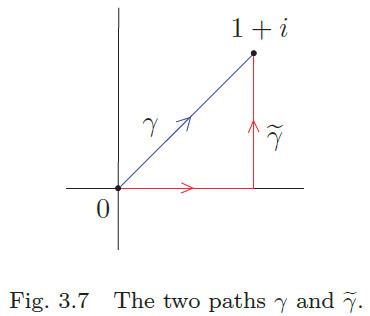
\includegraphics[width=0.4\textwidth]{./SaltChapter/fig-3-7}
\end{center}
\caption{두 경로 $\gamma$와 $\tilde\gamma$}
\label{fig-3-7}
\end{figure}
다른 적분 결과를 얻었다.
\[
\int_\gamma \bar z dz = 1 \ne 1+i = \int_{\tilde\gamma}\bar z dz.
\]
따라서 복소해석함수가 아닌 피적분함수 $z\to\bar z$는 경로에 따라 적분결과가 다르다.
경로적분의 정의를 보면
선택한 길에 따라 계산된 경로적분의 값이 다를 것으로 기대되기 때문에
결과가 이상하지는 않다.
이 장에서 중요한 목표는 
점 $z$에서 $w$까지 연결하는 두 경로 사이의 영역에서 복소해석적인 함수에 대하여
두 경로를 따라 적분한 결과는 동일함을 보이는 것이다.

















